\Chapter{Review of the literature}{Part I: Microelectronics design}
\label{cha:rol.icdesign}

\section{Introduction}

\section{3D integration}

The benefits of using 3D-ICs are numerous and have been already pointed out in the literature very often over the past few years \cite{659500}. First, by adding vertical dimension to the construction of the physical IC we can increase the IC packaging density. This means more gates for the same circuit footprint, that is much higher functional complexity of the final circuit for the same packaging volume. Secondly, the 3D-SICs are expected to have much better computing/power dissipation ratio. The integration in the 3rd dimension allows the design of circuits with different parts being closer to each other, resulting in less and shorter wires \cite{981091}. Lowering wire delays and allowing higher operating frequencies will result in increased bandwidths between nodes satisfying data hungry applications. Also, less and shorter wires mean lower total parasitic capacitance and inductance of the circuit, resulting in lower power dissipation. Finally, the 3D-SICs will enable the design of really heterogeneous systems, embedding not only traditional digital circuits such as processors and memories, but also analogue circuits such as sensors, antennas and power supplies \cite{4299568}.

Currently different technologies for fabrication of 3D-SICs have been proposed in the literature. Proposed methods have been used for implementation of complete systems going far beyond simple proof-of-concept or feasibility demonstrators. One can mention the implementation of a processor and memory in a single 3D chip dedicated for video coding applications \cite{1696226} and a processor with multiple levels of memory hierarchy dedicated for high-throughput server applications \cite{1168873}. Finally, the first commercial 3D-SIC products have been already announced by IBM \cite{1167715} and companies specialized in 3D semiconductor industry such as Tezzaron \cite{terra04}.

3D Integration is taken into account in the roadmaps of almost all key players in the field of integrated circuit design and manufacturing.

\subsubsection*{Interconnection length}

The 3D integration allows to design circuits with components closer to each other. Wire of a few millimetres long can be replaced by TSV of a few tens of microns \cite{659500}, as shown in Fig. \ref{fig:wire}. These shorter interconnections will introduce shorter delays, hence allowing higher working frequencies.

\begin{figure}[h!]
\begin{center}
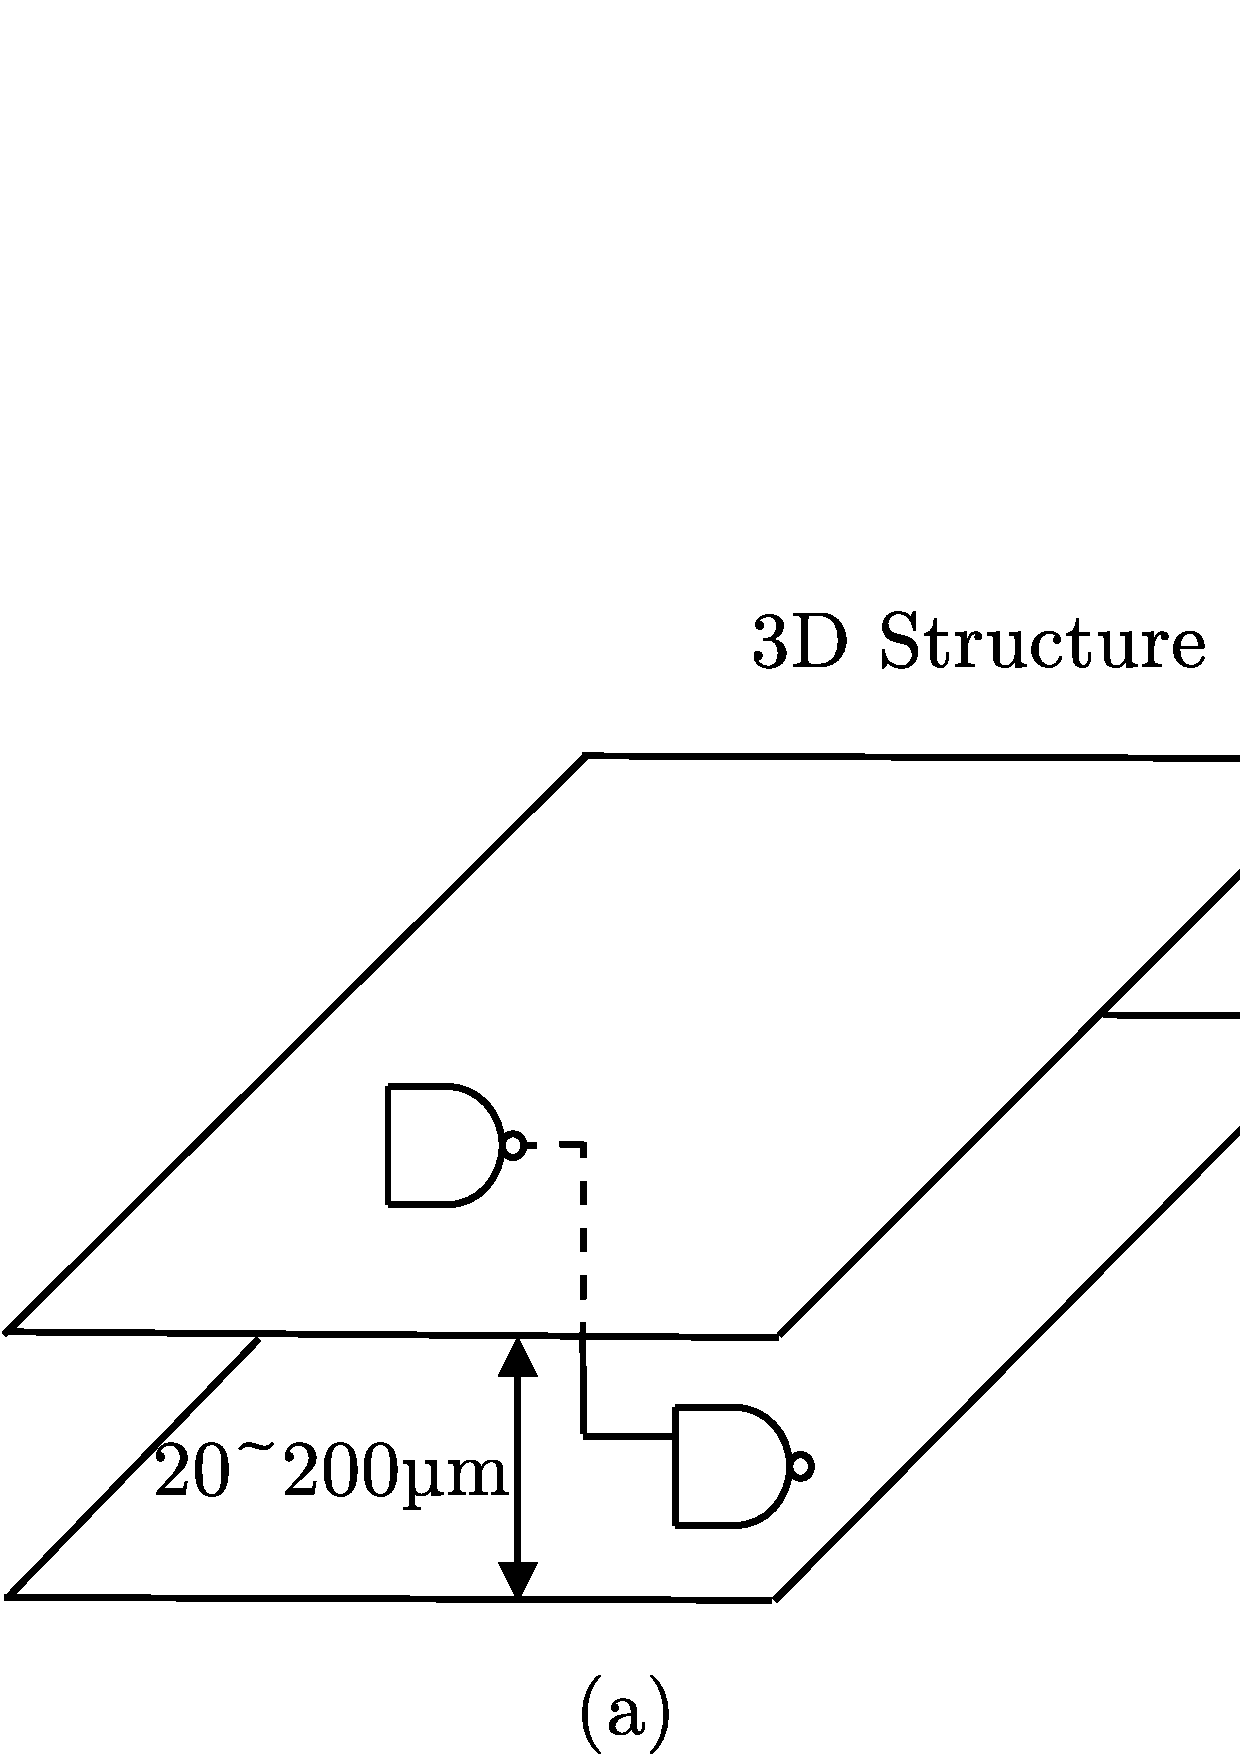
\includegraphics[width=0.75\linewidth]{wire.png}
\end{center}
\vspace{-0.5cm}
\caption{Shorter interconnections}
\label{fig:wire}
\end{figure}

\subsubsection*{Silicon efficiency and accessibility}

Adding a vertical dimension allows to increase the integration density. It is therefore possible to have more logic gates than a 2D-IC for the same footprint, hence a more efficient use of the silicon as shown in Fig. \ref{fig:footprint}. For instance, compared to the footprint of a 2D-IC, the 3D-SICs can double the integration for a 50\% use of a 2D footprint \cite{659500}.

\begin{figure}[h!]
\begin{center}
\includegraphics[width=0.75\linewidth]{footprint.png}
\end{center}
\vspace{-0.5cm}
\caption{Silicon efficiency}
\label{fig:footprint}
\end{figure}

In addition, the 3D integration allows a better accessibility for the components, as shown in Fig. \ref{fig:accessibility}. Indeed, for a 2D structure, 8 accessible neighbours can be considered for a central element (Fig. \ref{fig:accessibility} (a)), whereas for a 3D structure, the number of accessible neighbours can reach 116 (Fig. \ref{fig:accessibility} (b)) \cite{659500}.

\begin{figure}[h!]
\begin{center}
\includegraphics[width=0.75\linewidth]{accessibility.png}
\end{center}
\vspace{-0.5cm}
\caption{Components accessibility}
\label{fig:accessibility}
\end{figure}

\subsubsection*{Bandwidth}

The use of TSVs on 3D-SIC can significantly increase the bandwidth of a circuit. Indeed, as shown in Fig. \ref{fig:bandwidth}, the interconnections are not only limited to peripheral connections but can also make use of the circuit's surface. This increase of the bandwidth allows higher working frequencies so that it is easier to satisfy data-heavy applications.

\begin{figure}[h!]
\begin{center}
\includegraphics[width=0.75\linewidth]{bandwidth.png}
\end{center}
\vspace{-0.5cm}
\caption{Bandwidth improvement}
\label{fig:bandwidth}
\end{figure}

\subsubsection*{Consumption and noise}

Shorter interconnections generally translates into lower capacitance and inductance parasites. This means a decrease of the numbers of repeaters, hence a better consumption, less noise and less jitter.

\subsubsection*{Heterogeneous circuits}

The 3D technologies 
Les technologies 3D-SIC permettent le design de systèmes vraiment hétérogènes. Il est par exemple possible d'intégrer, en plus des circuits numériques traditionnels de technologies différentes, des circuits analogiques tels que des capteurs ou des antennes, et également des alimentations, ce qui confère aux 3D-SIC la possibilité d'avoir une très grande diversité fonctionnelle \cite{4299568}. À titre d'exemple, la Fig. \ref{fig:heterogeneity} illustre la vue schématique d'un 3D-SIC développé pour le secteur biomédical par IMEC qui contient des antennes, des DSP, 19 canaux de capteurs EEG/ECG, une alimentation, ainsi que des cellules photovoltaïques \cite{4198870}.

\begin{figure}[h!]
\begin{center}
\includegraphics[width=0.5\linewidth]{heterogeneity.png}
\end{center}
\vspace{-0.5cm}
\caption{Illustration schématique d'un 3D-SIC hétérogène (développé par IMEC) \cite{4198870}}
\label{fig:heterogeneity}
\end{figure}

\subsection{Technologies de fabrication}

Différentes technologies de fabrication de 3D-SIC ont été proposées dans la littérature et ont été utilisées pour des implémentations de systèmes complets, démontrant ainsi les réelles possibilités offertes par les 3D-SIC.

Parmi les technologies existantes, on peut en retenir quatre majeures qui illustrent de façon générale les méthodes d'intégration en 3D \cite{659500}.

\subsubsection*{\textit{Chip stacking}}

Cette méthode consiste à empiler des composants conçus et testés séparément pour produire un \textit{system-in-package} (SiP). Les composants empilés verticalement sont reliés entre eux par des fils de câblage traditionnels. L'avantage principal de cette méthode consiste en une réduction en taille. Les fils de connexion sont plus courts, mais les composants ne sont pas intégrés de façon plus dense par rapport à un système en 2D et la façon dont transitent les signaux est inchangée.

\subsubsection*{\textit{Transistor stacking}}

Le \textit{transistor stacking} consiste à créer plusieurs niveaux de transistors sur un seul substrat. C'est la meilleure méthode pour la conception de circuits 3D, mais les succès sont fortement limités actuellement à cause de problèmes liés à la thermique. Les températures requises pour graver une couche de transistors de haute performance provoqueraient la destruction du cuivre et de l'aluminium déjà déposés.

\subsubsection*{\textit{Die-on-wafer stacking}}

Dans cette méthode, des \textit{known good dies} (KGD, puce testée et fonctionnelle) sont reliés à un \textit{wafer} hôte contenant d'autres KGD. Les KGD peuvent être mis en connexion par des glues organiques, des liaisons d'oxyde ou métalliques. Le \textit{wafer} et les KGD qui y sont reliés sont ensuite affinés et mis en forme pour les interconnexions. Des substrats différents peuvent être combinés si la température de traitement est suffisamment basse pour minimiser les effets d'expansion non homogène.

Le \textit{die-on-wafer stacking} peut utiliser des interconnexions au niveau des bords des chips, des faces reliées ou à travers les chips. Selon le type d'interconnexions, cette méthode peut produire un niveau d'intégration nettement plus élevé que le \textit{chip stacking}, avec un meilleur rapport coût par connexion et une plus grande densité d'interconnexions, tout en gardant les avantages que présentent les KGD.

La qualité du \textit{stacking} dépend des équipements qui positionnent chaque chip sur son \textit{wafer}. La précision du placement détermine la densité d'interconnexions possible. Il faut également tenir compte du fait que les équipements actuels sont prévus pour manipuler des chips déjà entièrement conçus, et non des circuits nus, ce qui n'assure pas une protection adéquate aux décharges statiques.

\subsubsection*{\textit{Wafer-level stacking}}

Cette méthode consiste à relier des \textit{wafers} entiers entre eux pour former un \textit{stack}. Les connexions verticales passant à travers les \textit{wafers} sont établies directement à travers chaque substrat, vers le \textit{wafer} suivant et sa couche de transistors. Comme dans la méthode précédente, la densité d'interconnexions dépend fortement de la précision des équipements de placement, qui est cependant meilleure pour cette méthode, ce qui implique un coût moins élevé par interconnexion et une densité d'interconnexions plus grande par rapport au \textit{die-on-wafer stacking}.

Il est également possible de combiner des substrats différents, toujours en faisant attention à la température de traitement. Tous les procédés sont effectués au niveau du \textit{wafer}. Comme les équipements pour \textit{wafers} prévoient une protection aux décharges statiques, cela représente un avantage par rapport au \textit{die-on-wafer stacking}.

Il faut néanmoins faire attention au rendement des \textit{wafers} car toutes les puces présentes sur un \textit{wafer} ne sont pas forcément des KGD. Les méthodes pour relier deux \textit{wafers} ensemble sont les mêmes que celles pour relier deux KGD.
